\PassOptionsToPackage{unicode=true}{hyperref} % options for packages loaded elsewhere
\PassOptionsToPackage{hyphens}{url}
%
\documentclass[
]{article}
\usepackage{lmodern}
\usepackage{amssymb,amsmath}
\usepackage{ifxetex,ifluatex}
\ifnum 0\ifxetex 1\fi\ifluatex 1\fi=0 % if pdftex
  \usepackage[T1]{fontenc}
  \usepackage[utf8]{inputenc}
  \usepackage{textcomp} % provides euro and other symbols
\else % if luatex or xelatex
  \usepackage{unicode-math}
  \defaultfontfeatures{Scale=MatchLowercase}
  \defaultfontfeatures[\rmfamily]{Ligatures=TeX,Scale=1}
\fi
% use upquote if available, for straight quotes in verbatim environments
\IfFileExists{upquote.sty}{\usepackage{upquote}}{}
\IfFileExists{microtype.sty}{% use microtype if available
  \usepackage[]{microtype}
  \UseMicrotypeSet[protrusion]{basicmath} % disable protrusion for tt fonts
}{}
\makeatletter
\@ifundefined{KOMAClassName}{% if non-KOMA class
  \IfFileExists{parskip.sty}{%
    \usepackage{parskip}
  }{% else
    \setlength{\parindent}{0pt}
    \setlength{\parskip}{6pt plus 2pt minus 1pt}}
}{% if KOMA class
  \KOMAoptions{parskip=half}}
\makeatother
\usepackage{xcolor}
\IfFileExists{xurl.sty}{\usepackage{xurl}}{} % add URL line breaks if available
\IfFileExists{bookmark.sty}{\usepackage{bookmark}}{\usepackage{hyperref}}
\hypersetup{
  pdftitle={Reproducible Research: Peer Assessment 1},
  pdfborder={0 0 0},
  breaklinks=true}
\urlstyle{same}  % don't use monospace font for urls
\usepackage[margin=1in]{geometry}
\usepackage{color}
\usepackage{fancyvrb}
\newcommand{\VerbBar}{|}
\newcommand{\VERB}{\Verb[commandchars=\\\{\}]}
\DefineVerbatimEnvironment{Highlighting}{Verbatim}{commandchars=\\\{\}}
% Add ',fontsize=\small' for more characters per line
\usepackage{framed}
\definecolor{shadecolor}{RGB}{248,248,248}
\newenvironment{Shaded}{\begin{snugshade}}{\end{snugshade}}
\newcommand{\AlertTok}[1]{\textcolor[rgb]{0.94,0.16,0.16}{#1}}
\newcommand{\AnnotationTok}[1]{\textcolor[rgb]{0.56,0.35,0.01}{\textbf{\textit{#1}}}}
\newcommand{\AttributeTok}[1]{\textcolor[rgb]{0.77,0.63,0.00}{#1}}
\newcommand{\BaseNTok}[1]{\textcolor[rgb]{0.00,0.00,0.81}{#1}}
\newcommand{\BuiltInTok}[1]{#1}
\newcommand{\CharTok}[1]{\textcolor[rgb]{0.31,0.60,0.02}{#1}}
\newcommand{\CommentTok}[1]{\textcolor[rgb]{0.56,0.35,0.01}{\textit{#1}}}
\newcommand{\CommentVarTok}[1]{\textcolor[rgb]{0.56,0.35,0.01}{\textbf{\textit{#1}}}}
\newcommand{\ConstantTok}[1]{\textcolor[rgb]{0.00,0.00,0.00}{#1}}
\newcommand{\ControlFlowTok}[1]{\textcolor[rgb]{0.13,0.29,0.53}{\textbf{#1}}}
\newcommand{\DataTypeTok}[1]{\textcolor[rgb]{0.13,0.29,0.53}{#1}}
\newcommand{\DecValTok}[1]{\textcolor[rgb]{0.00,0.00,0.81}{#1}}
\newcommand{\DocumentationTok}[1]{\textcolor[rgb]{0.56,0.35,0.01}{\textbf{\textit{#1}}}}
\newcommand{\ErrorTok}[1]{\textcolor[rgb]{0.64,0.00,0.00}{\textbf{#1}}}
\newcommand{\ExtensionTok}[1]{#1}
\newcommand{\FloatTok}[1]{\textcolor[rgb]{0.00,0.00,0.81}{#1}}
\newcommand{\FunctionTok}[1]{\textcolor[rgb]{0.00,0.00,0.00}{#1}}
\newcommand{\ImportTok}[1]{#1}
\newcommand{\InformationTok}[1]{\textcolor[rgb]{0.56,0.35,0.01}{\textbf{\textit{#1}}}}
\newcommand{\KeywordTok}[1]{\textcolor[rgb]{0.13,0.29,0.53}{\textbf{#1}}}
\newcommand{\NormalTok}[1]{#1}
\newcommand{\OperatorTok}[1]{\textcolor[rgb]{0.81,0.36,0.00}{\textbf{#1}}}
\newcommand{\OtherTok}[1]{\textcolor[rgb]{0.56,0.35,0.01}{#1}}
\newcommand{\PreprocessorTok}[1]{\textcolor[rgb]{0.56,0.35,0.01}{\textit{#1}}}
\newcommand{\RegionMarkerTok}[1]{#1}
\newcommand{\SpecialCharTok}[1]{\textcolor[rgb]{0.00,0.00,0.00}{#1}}
\newcommand{\SpecialStringTok}[1]{\textcolor[rgb]{0.31,0.60,0.02}{#1}}
\newcommand{\StringTok}[1]{\textcolor[rgb]{0.31,0.60,0.02}{#1}}
\newcommand{\VariableTok}[1]{\textcolor[rgb]{0.00,0.00,0.00}{#1}}
\newcommand{\VerbatimStringTok}[1]{\textcolor[rgb]{0.31,0.60,0.02}{#1}}
\newcommand{\WarningTok}[1]{\textcolor[rgb]{0.56,0.35,0.01}{\textbf{\textit{#1}}}}
\usepackage{graphicx,grffile}
\makeatletter
\def\maxwidth{\ifdim\Gin@nat@width>\linewidth\linewidth\else\Gin@nat@width\fi}
\def\maxheight{\ifdim\Gin@nat@height>\textheight\textheight\else\Gin@nat@height\fi}
\makeatother
% Scale images if necessary, so that they will not overflow the page
% margins by default, and it is still possible to overwrite the defaults
% using explicit options in \includegraphics[width, height, ...]{}
\setkeys{Gin}{width=\maxwidth,height=\maxheight,keepaspectratio}
\setlength{\emergencystretch}{3em}  % prevent overfull lines
\providecommand{\tightlist}{%
  \setlength{\itemsep}{0pt}\setlength{\parskip}{0pt}}
\setcounter{secnumdepth}{-2}
% Redefines (sub)paragraphs to behave more like sections
\ifx\paragraph\undefined\else
  \let\oldparagraph\paragraph
  \renewcommand{\paragraph}[1]{\oldparagraph{#1}\mbox{}}
\fi
\ifx\subparagraph\undefined\else
  \let\oldsubparagraph\subparagraph
  \renewcommand{\subparagraph}[1]{\oldsubparagraph{#1}\mbox{}}
\fi

% set default figure placement to htbp
\makeatletter
\def\fps@figure{htbp}
\makeatother


\title{Reproducible Research: Peer Assessment 1}
\author{}
\date{\vspace{-2.5em}}

\begin{document}
\maketitle

\hypertarget{loading-and-preprocessing-the-data}{%
\subsection{Loading and preprocessing the
data}\label{loading-and-preprocessing-the-data}}

\begin{Shaded}
\begin{Highlighting}[]
\KeywordTok{download.file}\NormalTok{(}\StringTok{"https://d396qusza40orc.cloudfront.net/repdata%2Fdata%2Factivity.zip"}\NormalTok{, }\DataTypeTok{destfile =} \StringTok{"activity.zip"}\NormalTok{, }\DataTypeTok{mode=}\StringTok{"wb"}\NormalTok{)}
\KeywordTok{unzip}\NormalTok{(}\StringTok{"activity.zip"}\NormalTok{)}
\NormalTok{ActivityData <-}\StringTok{ }\KeywordTok{na.omit}\NormalTok{(}\KeywordTok{read.csv}\NormalTok{(}\StringTok{"activity.csv"}\NormalTok{, }\DataTypeTok{header =} \OtherTok{TRUE}\NormalTok{))}
\end{Highlighting}
\end{Shaded}

\hypertarget{what-is-mean-total-number-of-steps-taken-per-day}{%
\subsection{What is mean total number of steps taken per
day?}\label{what-is-mean-total-number-of-steps-taken-per-day}}

\begin{Shaded}
\begin{Highlighting}[]
\NormalTok{TotalSteps <-}\StringTok{ }\KeywordTok{aggregate}\NormalTok{(}\KeywordTok{as.numeric}\NormalTok{(ActivityData}\OperatorTok{$}\NormalTok{steps), }\DataTypeTok{by =} \KeywordTok{list}\NormalTok{(}\KeywordTok{as.numeric}\NormalTok{(ActivityData}\OperatorTok{$}\NormalTok{date)), }\DataTypeTok{FUN =} \StringTok{"mean"}\NormalTok{)}

\KeywordTok{hist}\NormalTok{(TotalSteps}\OperatorTok{$}\NormalTok{x, }\DataTypeTok{col =} \StringTok{"purple"}\NormalTok{,}
     \DataTypeTok{breaks =} \DecValTok{25}\NormalTok{,}
     \DataTypeTok{main =} \StringTok{"Total Number of Steps per Day"}\NormalTok{,}
     \DataTypeTok{xlab =} \StringTok{"Number of Steps"}\NormalTok{,}
     \DataTypeTok{ylab =} \StringTok{"Total Number per Day"}\NormalTok{)}
\end{Highlighting}
\end{Shaded}

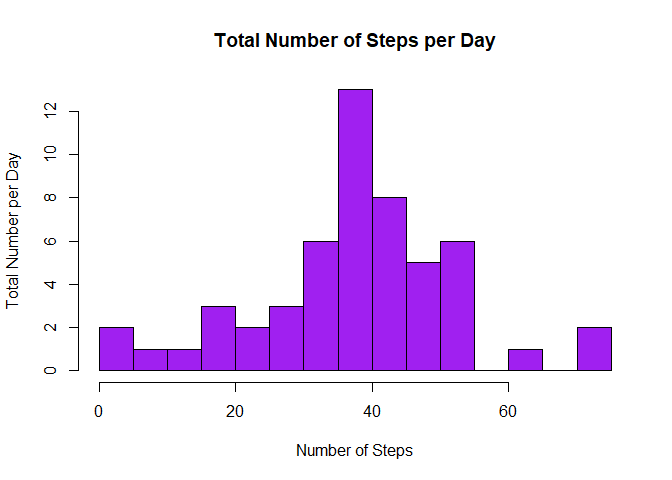
\includegraphics{PA1_Priscilla-Morales_files/figure-latex/unnamed-chunk-2-1.pdf}

\hypertarget{what-is-the-average-daily-activity-pattern}{%
\subsection{What is the average daily activity
pattern?}\label{what-is-the-average-daily-activity-pattern}}

\begin{Shaded}
\begin{Highlighting}[]
\NormalTok{MeanSteps <-}\StringTok{ }\KeywordTok{mean}\NormalTok{(TotalSteps[,}\DecValTok{2}\NormalTok{])}
\NormalTok{MedianSteps <-}\StringTok{ }\KeywordTok{median}\NormalTok{(TotalSteps[,}\DecValTok{2}\NormalTok{])}

\KeywordTok{print}\NormalTok{(MeanSteps)}
\end{Highlighting}
\end{Shaded}

\begin{verbatim}
## [1] 37.3826
\end{verbatim}

\begin{Shaded}
\begin{Highlighting}[]
\KeywordTok{print}\NormalTok{(MedianSteps)}
\end{Highlighting}
\end{Shaded}

\begin{verbatim}
## [1] 37.37847
\end{verbatim}

\begin{Shaded}
\begin{Highlighting}[]
\NormalTok{MeanStepsTS <-}\StringTok{ }\KeywordTok{aggregate}\NormalTok{(ActivityData}\OperatorTok{$}\NormalTok{steps, }\DataTypeTok{by =} \KeywordTok{list}\NormalTok{(ActivityData}\OperatorTok{$}\NormalTok{interval), }\DataTypeTok{FUN =} \StringTok{"mean"}\NormalTok{)}
\CommentTok{#hist(MeanStepsTS$x)}
\KeywordTok{plot}\NormalTok{(}\DataTypeTok{x =}\NormalTok{ MeanStepsTS}\OperatorTok{$}\NormalTok{Group}\FloatTok{.1}\NormalTok{, }\DataTypeTok{y =}\NormalTok{ MeanStepsTS}\OperatorTok{$}\NormalTok{x, }\DataTypeTok{type =} \StringTok{"l"}\NormalTok{,}
     \DataTypeTok{main =} \StringTok{"Average Number of Steps Taken Each Day"}\NormalTok{,}
     \DataTypeTok{col =} \StringTok{"purple"}\NormalTok{,}
     \DataTypeTok{xlab =} \StringTok{"Intervals"}\NormalTok{,}
     \DataTypeTok{ylab =} \StringTok{"Mean"}\NormalTok{)}
\end{Highlighting}
\end{Shaded}

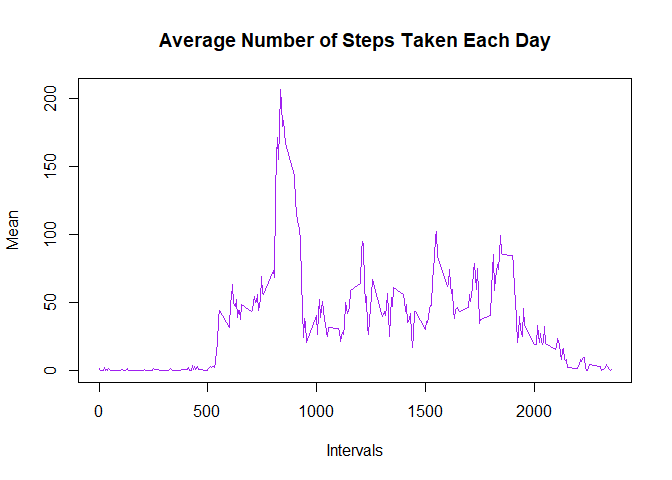
\includegraphics{PA1_Priscilla-Morales_files/figure-latex/unnamed-chunk-3-1.pdf}

\begin{Shaded}
\begin{Highlighting}[]
\CommentTok{#5 The 5-minute interval that, on average, contains the maximum number of steps}

\NormalTok{MeanStepsTS[}\KeywordTok{which}\NormalTok{(MeanStepsTS}\OperatorTok{$}\NormalTok{x}\OperatorTok{==}\StringTok{ }\KeywordTok{max}\NormalTok{(MeanStepsTS}\OperatorTok{$}\NormalTok{x)),]}
\end{Highlighting}
\end{Shaded}

\begin{verbatim}
##     Group.1        x
## 104     835 206.1698
\end{verbatim}

\hypertarget{imputing-missing-values}{%
\subsection{Imputing missing values}\label{imputing-missing-values}}

\begin{Shaded}
\begin{Highlighting}[]
\CommentTok{# 6 Code to describe and show a strategy for imputing missing data}
\CommentTok{# 6.1 Calculate the number of NAs}
\NormalTok{ActivityDataNAs <-}\StringTok{ }\KeywordTok{length}\NormalTok{(}\KeywordTok{which}\NormalTok{(}\KeywordTok{is.na}\NormalTok{(}\KeywordTok{read.csv}\NormalTok{(}\StringTok{"activity.csv"}\NormalTok{, }\DataTypeTok{header =} \OtherTok{TRUE}\NormalTok{))))}
\NormalTok{ActivityDataNAs}
\end{Highlighting}
\end{Shaded}

\begin{verbatim}
## [1] 2304
\end{verbatim}

\begin{Shaded}
\begin{Highlighting}[]
\NormalTok{AllActivityData <-}\StringTok{ }\NormalTok{(}\KeywordTok{read.csv}\NormalTok{(}\StringTok{"activity.csv"}\NormalTok{))}

\CommentTok{# 6.2 Filling Missing Values with Mean }

\KeywordTok{library}\NormalTok{(dplyr)}
\end{Highlighting}
\end{Shaded}

\begin{verbatim}
## Warning: package 'dplyr' was built under R version 3.6.3
\end{verbatim}

\begin{verbatim}
## 
## Attaching package: 'dplyr'
\end{verbatim}

\begin{verbatim}
## The following objects are masked from 'package:stats':
## 
##     filter, lag
\end{verbatim}

\begin{verbatim}
## The following objects are masked from 'package:base':
## 
##     intersect, setdiff, setequal, union
\end{verbatim}

\begin{Shaded}
\begin{Highlighting}[]
\NormalTok{ReplacingValues <-}\StringTok{ }\ControlFlowTok{function}\NormalTok{(x) }\KeywordTok{replace}\NormalTok{(x, }\KeywordTok{is.na}\NormalTok{(x), }\KeywordTok{mean}\NormalTok{(x, }\DataTypeTok{na.rm =} \OtherTok{TRUE}\NormalTok{))}
\NormalTok{MeanActivityDataNAs <-}\StringTok{ }\NormalTok{AllActivityData }\OperatorTok\StringTok{ }\KeywordTok{group_by}\NormalTok{(interval) }\OperatorTok\StringTok{ }\KeywordTok{mutate}\NormalTok{(}\DataTypeTok{steps =} \KeywordTok{ReplacingValues}\NormalTok{(steps))}


\CommentTok{# 6.3 Create new DataSet with Replacements}

\NormalTok{SummedActivityData <-}\StringTok{ }\KeywordTok{aggregate}\NormalTok{(MeanActivityDataNAs}\OperatorTok{$}\NormalTok{steps, }\DataTypeTok{by=}\KeywordTok{list}\NormalTok{(MeanActivityDataNAs}\OperatorTok{$}\NormalTok{date), sum)}
\KeywordTok{names}\NormalTok{(SummedActivityData)[}\DecValTok{1}\NormalTok{] =}\StringTok{"Date"}
\KeywordTok{head}\NormalTok{(SummedActivityData)}
\end{Highlighting}
\end{Shaded}

\begin{verbatim}
##         Date        x
## 1 2012-10-01 10766.19
## 2 2012-10-02   126.00
## 3 2012-10-03 11352.00
## 4 2012-10-04 12116.00
## 5 2012-10-05 13294.00
## 6 2012-10-06 15420.00
\end{verbatim}

\begin{Shaded}
\begin{Highlighting}[]
\CommentTok{# 7 Create a Histogram}

\KeywordTok{hist}\NormalTok{(SummedActivityData}\OperatorTok{$}\NormalTok{x,}
     \DataTypeTok{breaks =} \DecValTok{25}\NormalTok{,}
     \DataTypeTok{col =} \StringTok{"blue"}\NormalTok{,}
     \DataTypeTok{main =} \StringTok{"Replaced NAs Total Number of Steps per Day"}\NormalTok{)}
\end{Highlighting}
\end{Shaded}

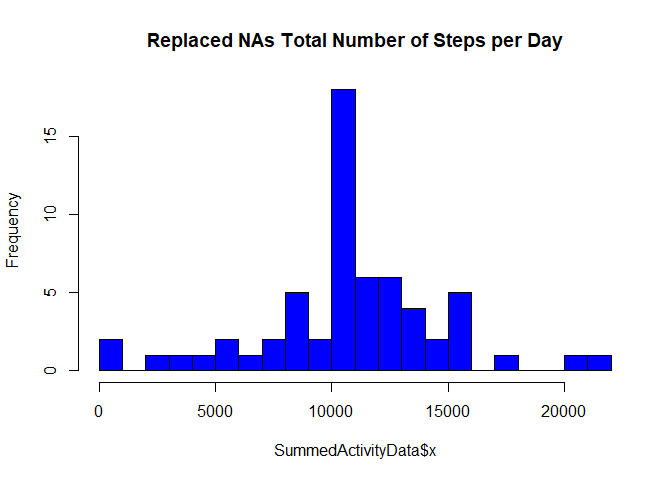
\includegraphics{PA1_Priscilla-Morales_files/figure-latex/unnamed-chunk-4-1.pdf}

\begin{Shaded}
\begin{Highlighting}[]
\CommentTok{# 7.1 Compare Central Metrics}

\NormalTok{MeanSteps <-}\StringTok{ }\KeywordTok{mean}\NormalTok{(TotalSteps[,}\DecValTok{2}\NormalTok{])}
\NormalTok{MedianSteps <-}\StringTok{ }\KeywordTok{median}\NormalTok{(TotalSteps[,}\DecValTok{2}\NormalTok{])}

\NormalTok{MeanSteps1 <-}\StringTok{ }\KeywordTok{mean}\NormalTok{(SummedActivityData}\OperatorTok{$}\NormalTok{x)}
\NormalTok{MedianSteps1 <-}\StringTok{ }\KeywordTok{median}\NormalTok{(SummedActivityData}\OperatorTok{$}\NormalTok{x)}

\NormalTok{MeanSteps}
\end{Highlighting}
\end{Shaded}

\begin{verbatim}
## [1] 37.3826
\end{verbatim}

\begin{Shaded}
\begin{Highlighting}[]
\NormalTok{MeanSteps1}
\end{Highlighting}
\end{Shaded}

\begin{verbatim}
## [1] 10766.19
\end{verbatim}

\begin{Shaded}
\begin{Highlighting}[]
\NormalTok{MedianSteps}
\end{Highlighting}
\end{Shaded}

\begin{verbatim}
## [1] 37.37847
\end{verbatim}

\begin{Shaded}
\begin{Highlighting}[]
\NormalTok{MedianSteps1}
\end{Highlighting}
\end{Shaded}

\begin{verbatim}
## [1] 10766.19
\end{verbatim}

\hypertarget{are-there-differences-in-activity-patterns-between-weekdays-and-weekends}{%
\subsection{Are there differences in activity patterns between weekdays
and
weekends?}\label{are-there-differences-in-activity-patterns-between-weekdays-and-weekends}}

\begin{Shaded}
\begin{Highlighting}[]
\CommentTok{# 8 Panel plot comparing the average number of steps taken per 5-minute interval across weekdays and weekends}
 
\NormalTok{MeanActivityDataNAs}\OperatorTok{$}\NormalTok{date <-}\StringTok{ }\KeywordTok{as.Date}\NormalTok{(MeanActivityDataNAs}\OperatorTok{$}\NormalTok{date)}
\NormalTok{MeanActivityDataNAs}\OperatorTok{$}\NormalTok{weekday <-}\StringTok{ }\KeywordTok{weekdays}\NormalTok{(MeanActivityDataNAs}\OperatorTok{$}\NormalTok{date)}
\NormalTok{MeanActivityDataNAs}\OperatorTok{$}\NormalTok{weekend <-}\StringTok{ }\KeywordTok{ifelse}\NormalTok{(MeanActivityDataNAs}\OperatorTok{$}\NormalTok{weekday}\OperatorTok{==}\StringTok{"Saturday"} \OperatorTok{|}\StringTok{ }\NormalTok{MeanActivityDataNAs}\OperatorTok{$}\NormalTok{weekday}\OperatorTok{==}\StringTok{"Sunday"}\NormalTok{, }\StringTok{"Weekend"}\NormalTok{, }\StringTok{"Weekday"}\NormalTok{ )}


\NormalTok{MeanActivityDataDays <-}\StringTok{ }\KeywordTok{aggregate}\NormalTok{(MeanActivityDataNAs}\OperatorTok{$}\NormalTok{steps , }\DataTypeTok{by=} \KeywordTok{list}\NormalTok{(MeanActivityDataNAs}\OperatorTok{$}\NormalTok{weekend, MeanActivityDataNAs}\OperatorTok{$}\NormalTok{interval), }\KeywordTok{na.omit}\NormalTok{(mean))}
\KeywordTok{names}\NormalTok{(MeanActivityDataDays) <-}\StringTok{ }\KeywordTok{c}\NormalTok{(}\StringTok{"weekend"}\NormalTok{, }\StringTok{"interval"}\NormalTok{, }\StringTok{"steps"}\NormalTok{)}


\KeywordTok{library}\NormalTok{(ggplot2)}
\end{Highlighting}
\end{Shaded}

\begin{verbatim}
## Warning: package 'ggplot2' was built under R version 3.6.3
\end{verbatim}

\begin{Shaded}
\begin{Highlighting}[]
\KeywordTok{ggplot}\NormalTok{(MeanActivityDataDays, }\KeywordTok{aes}\NormalTok{(}\DataTypeTok{x=}\NormalTok{interval, }\DataTypeTok{y=}\NormalTok{steps)) }\OperatorTok{+}\StringTok{ }\KeywordTok{geom_line}\NormalTok{()}\OperatorTok{+}
\StringTok{        }\KeywordTok{facet_grid}\NormalTok{(weekend }\OperatorTok{~}\NormalTok{.) }\OperatorTok{+}\StringTok{ }\KeywordTok{xlab}\NormalTok{(}\StringTok{"Interval"}\NormalTok{) }\OperatorTok{+}\StringTok{ }\KeywordTok{ylab}\NormalTok{(}\StringTok{"Mean of Steps"}\NormalTok{) }\OperatorTok{+}
\StringTok{        }\KeywordTok{ggtitle}\NormalTok{(}\StringTok{"5-minute interval across weekdays and weekends"}\NormalTok{)}
\end{Highlighting}
\end{Shaded}

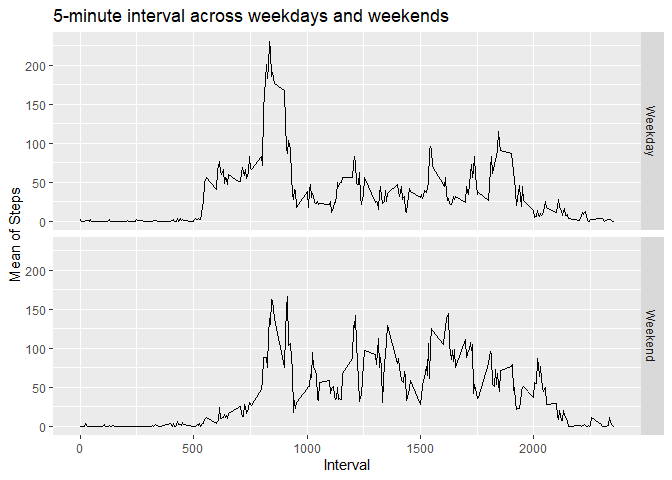
\includegraphics{PA1_Priscilla-Morales_files/figure-latex/unnamed-chunk-5-1.pdf}

\end{document}
